\section{Theoretische Grundlagen}


\subsection{Radioaktivität}
\subsubsection{$\alpha$-Zerfall}

Zerfällt ein sogenannter Mutterkern $_Z^AX$ in einen Tochterkern $_{Z-2}^{A-4}Y$ und ein $He^{2+}$-Ion so spricht man von $\alpha$-Zerfall. Das $He^{2+}$-Teilchen wird $\alpha$-Teilchen genannt. Die Emission von $\alpha$-Teilchen ist ein quantenmechanischer Prozess, der durch Tunneln des $\alpha$-Teilchens durch die Potentialbarriere des Coulombpotentials des Kerns ermöglicht wird. $\alpha$-Teilchen zeigen ein diskretes Spektrum. Der $\alpha$-Zerfall ist für den Versuch nicht von Relevanz.

\subsubsection{$\beta$-Zerfall}

Man unterscheidet beim $\beta$-Zerfall zwischen $\beta^+$- und $\beta^-$-Zerfall und dem Elektroneneinfang.

\begin{figure}[H]
	\begin{minipage}{0.5\textwidth}
	\centering 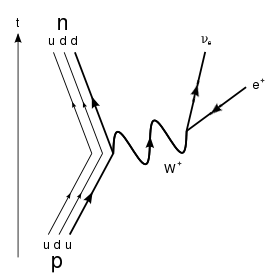
\includegraphics[width=\textwidth]{BilderTheorie/betaplus.png}
	\caption{$\beta^+$-Zerfall [en.wikipedia.org]}
	\end{minipage}
	\begin{minipage}{0.5\textwidth}
	\centering 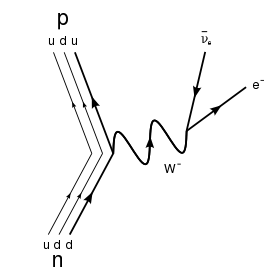
\includegraphics[width=\textwidth]{BilderTheorie/betaminus.png}
	\caption{$\beta^-$-Zerfall  [en.wikipedia.org]}	
	\end{minipage}
\end{figure}

Der $\beta^+$-Zerfall ist die Umwandlung eines Protons in ein Neutron mit Emission eines Positrons und eines Elektronenneutrinos:

$$ \beta^+: p^+ \rightarrow n^0 + e^+ + \nu_e $$

Dieser Zerfall ist wichtig für den Versuch, da auf diese Art Positronen erzeugt werden können, die mit Elektronen einen gebundenen Zustand eingehen können, nämlich das Positronium, welches in \ref{1} näher behandelt wird.
Der $\beta^-$-Zerfall ist die Umwandlung eines Neutrons in ein Proton, unter Emission eines Elektrons und eines Elektronen-Antineutrinos:

$$ \beta^-: n^0 \rightarrow p^+ + e^- + \bar \nu_e $$

Der $\beta^+$-Zerfall ist nur möglich für Protonen in einem Kern, da durch die Bindungsenergie die für den Prozess nötige Energie aufgebracht werden kann. Freie Protonen sind stabil.

Als weitere Art des $\beta$-Zerfall zählt man noch den Elektroneneinfang (EC, \emph{electron capture)}. Dieser kann stattfinden, wenn ein Elektron der untersten Schale (K-Schale), wegen dessen Aufenthaltswahrscheinlichkeit im Kern, vom Kern eingefangen wird und mit einem Proton zu einem Neutron reagiert. Dabei wird ein Elektronenneutrino emittiert:

$$ EC: p^+ + e^- \rightarrow n^0 + \nu_e $$

Der Elektroneneinfang gewinnt mit größeren Kernzahlen an Bedeutung, da dann die Aufenthaltswahrscheinlichkeit im Kern immer größer wird.

\subsubsection{$\gamma$-Zerfall}

Beim $\alpha$- und $\beta$-Zerfall gehen die Mutterkerne mit bestimmten Wahrscheinlichkeiten in verschiedene Anregungszustände der Tochterkerne über. Letztere zerfallen innerhalb einer sehr kurzen Zeit ($\sim 10^{-9}$ bis $10^{-12} s$) in den Grundzustand und emittieren dabei ein Photon mit Energien über 120 keV genannt $\gamma$-Quanten. Dieses $\gamma$-Quant wird entweder direkt vom Kern emittiert oder kann durch innere Konversion oder den Auger-Effekt seine Energie an Elektronen abgeben.

\subsection{Wechselwirkung von Photonen mit Materie \label{2}}

\subsubsection{Das Absorptionsgesetz}

Ein Photonenstrahl der einfallenden Intensität $I_0$ nimmt exponentiell mit der Dicke x einer durchquerten Materieschicht an Intensität ab. Es gilt also:

$$ I = I_0\cdot e^{-\mu x} $$

wobei $\mu$ der mediumabhängige (und photonenenergieabhängige) Absorptionkoeffizient ist. $\mu$ lässt sich als Summe der Absorptionskoeffizienten aller möglichen Wechselwirkungen von Photonen mit Materie schreiben, nämlich des Photoeffekts, des Compton-Effekts und der Paarbildung.

$$\mu = \mu_{Ph.} + \mu_{C} + \mu_{PB} $$

\subsubsection{Der Photoeffekt}

\begin{figure}[H]
	\begin{minipage}{0.59\textwidth}
	\centering 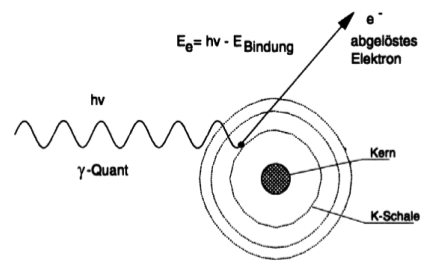
\includegraphics[width=\textwidth]{BilderTheorie/Photoeffekt.png}
	\caption{Photoeffekt}
	\end{minipage}
	\begin{minipage}{0.4\textwidth}
	Wenn ein $\gamma$-Quant ein Elektron aus der Atomhülle herausschlägt, spricht man vom Photoeffekt. Dieser Effekt tritt nur an gebundenen Elek\-tro\-nen auf. Die Energie des Photons geht zum größten Teil auf das Elektron, ein Teil wird jedoch als Rückstoßenergie vom Atom aufgenommen. Die Ab\-sorp\-tions\-wahrscheinlichkeit ist am größten in der K-Schale, also näher beim Kern. Der Photoeffekt dominiert gegenüber den anderen Effekten vor allem bei großen Atomen und Energien unter 100keV des Photons. Die entstandene Lücke wird dann durch ein weniger stark gebundenes oder freies Elektron aufgefüllt, wobei die Differenz der Bindungsenergien als Photon emittiert wird.
	\end{minipage}
\end{figure}

\subsubsection{Der Compton-Effekt}

\begin{figure}[H]
	\begin{minipage}{0.4\textwidth}
	Trifft ein Photon auf ein leicht gebundenes oder freies Elektron, so wird das Photon nicht ganz absorbiert, sondern gibt einen Teil seiner Energie an das Elektron ab und wird selbst gestreut. Durch die Streuung verliert das Photon somit an Energie, d.h. die Frequenz des gestreuten Quants ist kleiner. Der Compton-Effekt dominiert bei Energien zwischen 100 keV und einigen MeV.
	\end{minipage}
	\begin{minipage}{0.59\textwidth}
	\centering 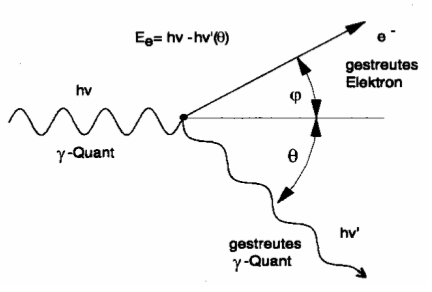
\includegraphics[width=\textwidth]{BilderTheorie/Comptoneffekt.png}
	\caption{Comptoneffekt}
	\end{minipage}

\end{figure}

\subsubsection{Die Paarbildung}

\begin{figure}[H]
	\begin{minipage}{0.5\textwidth}
	\centering 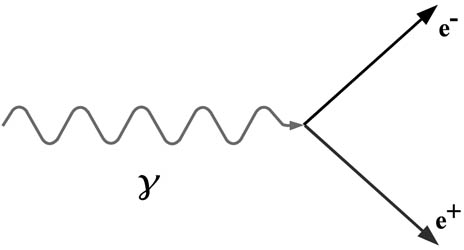
\includegraphics[width=\textwidth]{BilderTheorie/Paarbildung.jpg}
	\caption{Paarbildung}
	\end{minipage}
	\begin{minipage}{0.5\textwidth}
	Hat der $\gamma$-Quant mindestens die doppelte Ruheenergie eines Elektrons, also 1.022 MeV, so kann dieses im Feld eines Atomkerns (Stoßpartner für die Energie-Impuls-Erhaltung) ein Elektron-Positron-Paar erzeugen. 
	\end{minipage}
\end{figure}


\subsection{Szintillationszähler}

\begin{figure}[H]
	\centering 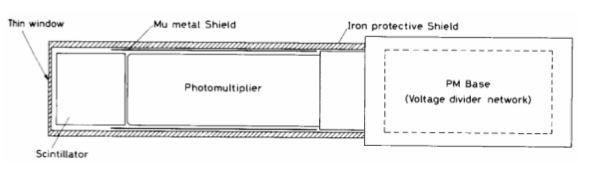
\includegraphics[width=\textwidth]{BilderTheorie/Szinti.png}
	\caption{Schema eines Szintillationszählers}
\end{figure}

Ein Szintillationszähler benutzt die in \ref{2} erklärten Ionisierungs-Phänomene um Photonen anhand geladener Strahlung nachzuweisen. Die geladene Strahlung löst Lichtblitze aus, die an einer Photokathode im Szintillator Elektronen freisetzen (Photoeffekt). Diese werden wiederum durch einen Photomultiplier verstärkt, so dass sie ein Signal mit einer messbaren Amplitude herausgeben, die der Energie des eingefallenen Quants proportional ist. Man unterscheidet zwischen organischen und anorganischen Szintillatoren. Bei dem organischen werden einzelne Moleküle angeregt, welche messbare Quanten emittieren. Beim anorganischen entstehen diese in einem Kristallgitter. Im Versuch benutzen wir anorganische NaI-Szintillationszähler.

\begin{figure}[H]
	\begin{minipage}{0.45\textwidth}
	Das Bändermodell erlaubt eine einfache Beschreibung des Verhaltens. Nämlich befinden sich bei tiefen Temperaturen alle Elektronen des Kristalls im sogenannten Valenzband. Absorbieren diese Elektronen energiereiche Strahlung, z.B. durch $\gamma$-Quanten (v.a. Photoeffekt), so werden diese angeregt und steigen auf höhere Energieniveaus. Reicht die Energie aus, so werden die Elektronen ins Leitungsband gehoben. Falls sie nicht groß genug ist um das Elektron vom Valenzband ins Leitungsband zu heben, so können sogenannte Exzitonen entstehen, lose gekoppelte Elektron-Loch-Paare (siehe Abb \ref{baendermodellszinti}). Die Exzitonen, können sich genau so wie die Leitungsband-Elektronen frei im Kristall bewegen und können unter Emission eines Photons wieder in den Grundzustand zurückkehren. 
	\end{minipage}
	\begin{minipage}{0.54\textwidth}
	\centering 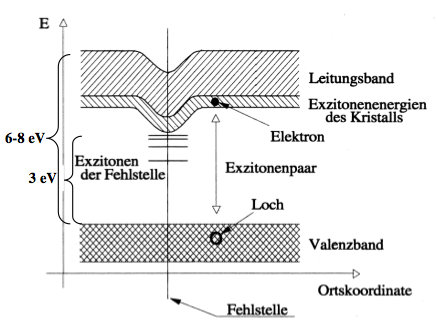
\includegraphics[width=\textwidth]{BilderTheorie/Bandmodell.png}
	\caption{Bändermodell beim NaI:Tl$^+$}
	\label{baendermodellszinti}
	\end{minipage}
\end{figure}
Eintreffende $\gamma$-Quanten haben Energien im Bereich von 0.1 bis 1 MeV, regen also mehrere hundert Elektronen gleichzeitig an. Wenn diese Elektron-Loch-Paare rekombinieren, entstehen neue Photonen, welche in den Photomultiplier geraten und dort verstärkt werden. Die Dotierung verformt lokal das Leitungsband und da diese Photonen vor allem an den Tl-Störstellen rekombinieren, reicht ihre Energie nicht aus um andere Elektronen ins Leitungsband anzuregen, somit können die Photonen nicht wieder vom Kristall absorbiert werden.


\subsection{Das Positronium \label{1}}

\begin{figure}[H]
	\begin{minipage}{0.5\textwidth}
	\centering 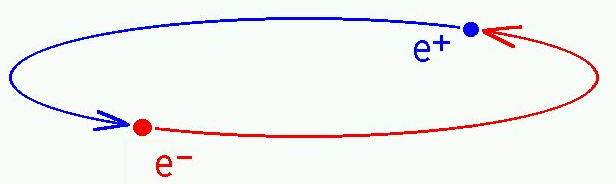
\includegraphics[width=0.9\textwidth]{BilderTheorie/Positronium.png}
	\caption{Das Positronium [cs.cdu.edu.au]}
	\end{minipage}
	\begin{minipage}{0.5\textwidth}
	Ein Positronium ist ein gebundener Zustand zwischen einem Elektron $e^-$ und dessen Antiteilchen, einem Positron $e^+$. Man kann es sich wie ein Wasserstoffatom vorstellen, bei dem das Proton durch das Positron vertauscht wurde. Der Schwerpunkt befindet sich in der Mitte der beiden Teilchen und somit ist die reduzierte Masse nur etwa halb so groß wie beim Wasserstoffatom, also genau die halbe Elektronen- bzw. Positronenmasse.
	\end{minipage}
\end{figure}
Die Energieniveaus (ohne Feinstruktur etc.) im Positronium sind also durch folgende Formel gegeben:

\begin{equation} E_n = -\frac{Ry}{2}\frac{1}{n^2} \label{3} \end{equation}

Wie man leicht nachrechnen kann, ist somit die Bindungsenergie des Grundzustands 6.8 eV, und die des 1. angeregten Zustands nur noch 1.7 eV.

\subsubsection{Erzeugung}

Ein Positron in Materie wird an den Atomen bzw. Molekülen gestreut und gibt somit einen großen Teil seiner kinetischen Energie ab. Kommt es zu einer Kollision mit einem Elektron, so annihilieren beide Teilchen. Ist die Energie des Positrons jedoch klein genug, so kann er wegen der Coulombkraft mit einem Elektron in einer äußeren Schale eines Atoms eine Bindung eingehen (Positronium), dessen Lebensdauer sich etwa im Nanosekunden-Bereich befindet und schließlich auch in einer Annihilation der beiden Teilchen endet. Mithilfe der Formel (\ref{3}), kann man erkennen, dass die Energie der Positronen über $V_i - 6.8$ eV sein muss, damit ein Positronium im Grundzustand erzeugt werden kann ($V_i$ ist die Ionisationsenergie der Atome oder Moleküle des Mediums). Die Erzeugung des 1. angeregten Zustands ist sehr unwahrscheinlich, da bei den betroffenen Energien die inelastische Streuung stark überwiegt. 

Die Annihilation unterscheidet sich je nach Spinstellung der beiden Teilchen, nämlich zerfallen sie entweder in 2 oder 3 Photonen.
Der Wirkungsquerschnitt für den 2$\gamma$-Zerfall ist gegeben durch

\begin{equation} \sigma_{2\gamma}=\frac{\pi\cdot r_0^2\cdot c}{v} \end{equation}

wobei $r_0=e^2/mc^2=2.8 fm$ der Thomson-Radius (klassischer Elektronenradius) ist und $v$ die Relativgeschwindigkeit zwischen dem Elektron und dem Positron. Der Wirkungsquerschnitt für den 3$\gamma$-Zerfall ist um $\alpha=1/137$ (Feinstrukturkonstante) kleiner. Auf die Spinstellungen und deren Unterschiede wird im nächsten Punkt näher eingegangen.

\subsubsection{Para- und Orthopositronium}

Da das Elektron und das Positron beide einen Spin von $j=1/2$ haben, können sie im gebundenen Zustand entweder zu einem Singulett oder zu einem Triplett koppeln.\\

\begin{tabular}[H]{p{4cm} p{4cm} p{4cm}}
 & Para-Positronium & Ortho-Positronium\\
 & &\\
Zustand & Singulett $^1S_0$ & Triplett $^3S_1$\\
Spineinstellung & Antiparallel, $J=0$ & Parallel, $J=1$\\
 & $m_J = 0$ & $m_J = -1,\ 0,\ 1$\\
Hauptzerfall & 2$\gamma$ & 3$\gamma$\\
Lebensdauer & $1.25\cdot 10^{-10} s$ & $1.39\cdot 10^{-7} s$\\
\end{tabular}\\

Der 1$\gamma$-Zerfall ist wegen der Impulserhaltung nicht möglich. Zerfälle in mehr als 3 Photonen sind durchaus möglich, wobei das Para-Positronium nur in eine gerade Zahl Photonen zerfallen kann und das Ortho-Positronium nur in ungerade Zahlen (siehe hierzu Kap. \ref{4}). Höhere Zerfälle sind jedoch relativ unwahrscheinlich und irrelevant für die Messung.
Der Unterschied in der Lebensdauer beträgt den Faktor:

\begin{equation} \frac{\tau_{2\gamma}}{\tau_{3\gamma}} = 1115 \end{equation}

\subsubsection{Auswahlregeln der Zerfälle \label{4}}

Um die Symmetrieauswahlregeln der Zerfälle der beiden Positronium-Zustände zu bestimmen, benutzen wir die C-Parität. Wir beweisen zuerst kurz, dass die Ladungskonjugation $\hat C$ auf ein Positronium angewandt genau die gleiche Operation macht, als würde man zuerst den Paritäts-Operator $\hat P$ und dann den Spinaustausch-Operator $\hat S$ auf das Positronium anwenden.

Man habe zum Beispiel ein Elektron am Ort $\vec r$ mit Spin $\alpha$ und ein Positron mit Ort $-\vec r$ und dem Spin $\beta$:
$$\hat S\cdot\hat P\mid e^-,\ \vec r,\ \alpha \rangle \otimes \mid e^+,\ -\vec r,\ \beta \rangle
 = p\hat S\mid e^-,\ -\vec r,\ \alpha \rangle \otimes \mid e^+,\ \vec r,\ \beta \rangle 
 = sp\mid e^-,\ -\vec r,\ \beta \rangle \otimes \mid e^+,\ \vec r,\ \alpha \rangle $$
Wie man sieht entspricht der Endzustand genau der Ladungskonjugation der beiden Teilchen, also direkt der Ersetzung der beiden Teilchen durch ihr Antiteilchen. Der Eigenwert sp entspricht somit dem Eigenwert c. Diese Ersetzung macht man, um die Eigenwerte der Ladungskonjugation zu bestimmen.

Da die Parität des Elektrons genau der Parität des Positrons entgegengesetzt ist, folgt für den Eigenwert
$$p = -(-1)^l = -1 \text{\ \ im Grundzustand (l=0)}$$
Der Eigenwert des Spinaustauschoperators ist gegeben durch $$s=(-1)^{J+1}$$
Somit ist $s=-1$ für den Singulett-Zustand und $s=1$ für den Triplett-Zustand.
Schlussendlich gilt also:

\begin{equation} \hat C \mid ^1S_0 \rangle = 1 \mid ^1S_0 \rangle \end{equation}
\begin{equation} \hat C \mid ^3S_1 \rangle = -1 \mid ^1S_0 \rangle \end{equation}

Die Photonen, die beim Zerfall ausgestrahlt werden, besitzen die C-Parität -1. Somit hat ein n-Photonen-Zerfall die Parität $(-1)^n$, was erklärt, warum der Singulett-Zustand nur in 2n Photonen und der Triplett-Zustand nur in 2n+1 Photonen zerfallen kann.

\subsubsection{Hyperfeinstruktur und Annihilationskraft \label{5}}

Der Hamiltonian der ''Grobstruktur'' lautet $$H = \frac{p_{e^-}^2}{2m_e}+\frac{p_{e^+}^2}{2m_e}-\frac{e}{r^2}$$ woraus die Energiezustände in Gl. (\ref{4}) folgen. Wenn man neben der Feinstruktur auch noch die Wechselwirkungen der magnetischen Spinmomente betrachtet, die sogenannte Hyperfeinstruktur, stößt man auf eine Energieaufspaltung der Triplett und Singulettzustände im Grundzustand. Neben der Hyperfeinstruktur spielt auch noch die Annihilationskraft eine genau so große Rolle in der Aufspaltung dieser Niveaus.

\begin{itemize}

\item Hyperfeinstruktur:\\
Die Wechselwirkungsenergie der magnetischen Momente entspricht in erster Näherung
\begin{equation} W = \frac{8\pi}{3}\mu^2\sigma^-\sigma^+|\Psi(0)|^2 \end{equation}
wobei $\sigma^\pm$ die Spinzustände des Positrons/Elektrons sind und $\mu = \frac{e\hbar}{2mc}$ das Bohrsche Magneton. $\Psi(0)$ ist die Wellenfunktion am Ort des Positron und ihr Betragsquadrat ist
$$|\Psi(0)|^2 = \frac{1}{\pi}\left(\frac{-1}{2a_0}\right)^3$$
$a_0 = 0.53 \mathring A$ ist der Bohrsche Atomradius. Der Eigenwert des Spinoperators $\sigma^-\sigma^+$ beträgt für den Singulett-Zustand -3 und für den Triplett-Zustand +1. Man erhält somit die Energiebeiträge
$$W(^1S_0) = -\frac{1}{4}\alpha^4mc^2 \text{\ \ \ \ und \ \ \ \ } W(^3S_1) = \frac{1}{12}\alpha^4mc^2$$
und kann ausrechnen dass die Aufspaltung
\begin{equation} \Delta W = 4.83 \cdot 10^{-4}\ eV \end{equation} beträgt, und der Triplett-Zuständ oberhalb des Singulett-Zustands liegt.

\item Annihilationskraft:\\
\begin{figure}[H]
	\begin{minipage}{0.5\textwidth}
	Die sogenannte Annihilationskraft berücksichtigt den Fall, dass ein Elektron und ein Positron kurzzeitig in ein virtuelles Photon annihilieren können und dann wieder ein Positronium bilden können. Diese Tatsache liefert einen Energieterm für alle Zustände mit ungerader C-Parität, da nur diese in eine ungerade Zahl Photonen zerfallen können (siehe vorigen Abschnitt). Der Triplettzustand erhält hierdurch den Energiebeitrag:

\begin{equation} W_A(^3S_1)=8\pi\mu^2|\Psi(0)|^2 = \frac{1}{4}\alpha^2mc^2 \end{equation}

Der numerische Wert hierfür ist $W_A = 3.62\cdot10^{-4}$ eV und ist somit fast genau so groß wie der Term der Hyperfeinstruktur.
	\end{minipage}
	\begin{minipage}{0.5\textwidth}
	\centering 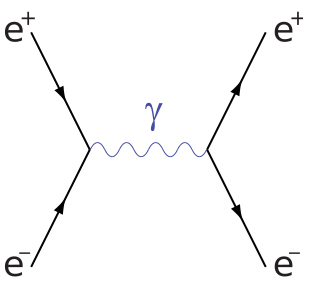
\includegraphics[width=0.8\textwidth]{BilderTheorie/epep.png}
	\caption{Feynman-Graph der Annihila\-tionskraft [howgravityworks.org]}
	\end{minipage}
\end{figure}

\item Die gesamte Aufspaltung beträgt somit 
\begin{equation} \boxed{\Delta W = \frac{7}{12}\alpha^4mc^2 = 8.45\cdot10^{-4} eV} \end{equation}
\end{itemize}

\subsection{Der Zeeman-Effekt}

Der Zeeman-Effekt beschreibt die Aufspaltung der Energiezustände eines gebundenen Zustands in einem Magnetfeld B. Man unterscheided zwischen dem normalen und dem anomalen Zeeman-Effekt. 
Der normale Zeeman-Effekt spaltet die Energieniveaus eines bestimmten Bahndrehimpulses $l$ in $2l+1$ Terme, deren Energieaufspaltung abhängig von der z-Komponente $m_l$ des Bahdrehimpulses ist:
$$\Delta E = \mu_B\cdot m_l \cdot B$$
$\mu_B$ ist hier das Bohrsche Magneton. Der normale Zeeman-Effekt ist also die Aufspaltung aufgrund des mit dem Bahndrehimpulses verknüpften magnetischen Moment in einem externen Magnetfeld.
Der anomale Zeeman-Effekt ist die zusätzliche Berücksichtigung des magnetischen Moments, das durch den Spin hervorgerufen wird. Hier muss also die $l-s$-Kopplung ($\vec J = \vec L + \vec S$) berücksichtigt werden, so dass die Aufspaltung
$$\Delta E = g_J\cdot\mu_B\cdot m_J\cdot B$$
beträgt, wobei $g_J$ der Landé-Faktor des Gesamtdrehimpulses ist.\\

Das Positronium selber hat kein magnetisches Moment, da sich das vom Elektron mit dem vom Positron genau aufhebt. Da jedoch das externe Magnetfeld im Positronium ein magnetisches Moment erzeugt, kann dieses wiederum vom Magnetfeld aufgespalten werden, so dass man einen Zeeman-Effekt 2. Ordnung erhält. Dieser ist im Allgemeinen wesentlich schwächer als der Zeeman-Effekt 1. Ordnung, ist aber beim Positronium der einzige der beiträgt. Das Magnetfeld fließt quadratisch in die Aufspaltung ein. Die Wirkung des Effekts lässt sich mittels quantenmechanischer Störungstheorie berechnen. Der Störungsoperator hat die Form:

\begin{equation} V=\frac{e\hbar B}{2mc}(\sigma^- - \sigma^+) \end{equation} 

Wendet man diesen Operator auf die Spinwellenfunktionen $\ket{S,m_s}$ der Singulett- und Triplett-Zustände an, erhält man (ohne Vorfaktoren):\\

\begin{tabular}[H]{l l l}
Singulett 	& $(\sigma^- - \sigma^+)\ket{0,0}$ &$ = 2\ket{1,0}$\\
& & \\
		& $(\sigma^- - \sigma^+)\ket{1,-1}$ & $ = 0$\\
Triplett 	& $(\sigma^- - \sigma^+)\ket{1,0}$ &$ = 2\ket{0,0}$\\
		& $(\sigma^- - \sigma^+)\ket{1,1}$ &$ = 0$\\
\end{tabular}\\

Wie man sehen kann, werden die $m_S = 1$-Zustände nicht vom Magnetfeld beeinflusst, da ihr Eigenwert 0 ist. Die $m_S = 0$-Zustände werden gemischt, d.h. $\bra{1,0}V\ket{0,0}\neq 0$ bei Anwesenheit eines externen Magnetfelds. Man benutzt nun die Schrödingergleichung mit dem Hamiltonoperator $H=\frac{p^2}{2m}+V$ um die Energieeigenwerte der beiden von der Störung betroffenen Zustände zu bestimmen. Die auf diesem Wege erhaltenen Energien sind:

\begin{equation} \text{Singulett\ \ \ } E_{\ket{0,0}} = \frac{1}{2}(E_{\ket{0,0}}^{(0)} - E_{\ket{1,0}}^{(0)}) - \frac{1}{2}\Delta E^{(0)}\sqrt{1+x^2} \end{equation}
\begin{equation} \text{Triplett\ \ \ \ \ } E_{\ket{1,0}} = \frac{1}{2}(E_{\ket{0,0}}^{(0)} + E_{\ket{1,0}}^{(0)}) + \frac{1}{2}\Delta E^{(0)}\sqrt{1+x^2} \end{equation}

Wobei gilt:

$$ E^{(0)} \text{ : Energie des ungestörten Hamiltonian \ } $$
$$ \Delta E^{(0)} = E_{\ket{1,0}}^{(0)} - E_{\ket{0,0}}^{(0)} $$
\begin{equation} x = \frac{2e\hbar B}{mc\Delta E^{(0)}} \end{equation} \\

Man sieht also an oberen Energieeigenwerten, dass die Zustände $\ket{1,0}$ und $\ket{0,0}$ im Magnetfeld noch weiter aufgespaltet werden, also zusätzlich zu der in Abschnitt \ref{5} berechneten Aufspaltung. Die Abhängigkeit vom Magnetfeld ist quadratisch, da $x\sim B$ und $x$ quadratisch in die Gleichung einfließt.

\begin{figure}[H]
\centering 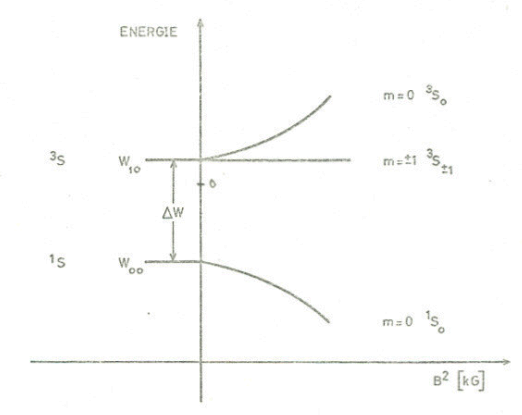
\includegraphics[width=\textwidth]{BilderTheorie/Zeeman.png}
\caption{Zeeman-Aufspaltung der Zustände [Staatsexamensarbeit von V.Bündge]}
\end{figure}

\subsection{Das Quenching}

Wie schon im vorigen Kapitel beschrieben, werden unter Einfluss eines externen Magnetfelds die $m_S = 0$-Zustände gemischt, sind also nicht mehr unabhängig voneinander. Man erhält das nicht-verschwindende, nichtdiagonale Matrixelement 

$$ M = \bra{1,0} V \ket{0,0} = \frac{e\hbar B}{mc} $$

\subsubsection{Störungsrechnung}

Man versucht nun den genauen Einfluss des Magnetfelds störungstheoretisch zu berechnen. Man löst die zeitabhängige Schrödingergleichung

$$ i\hbar \frac{d\Psi}{dt} = (\frac{p^2}{2m}+V)\Psi $$

mit dem allgemeinen Ansatz:

$$ \Psi = \sum_{k} b_k(t)\Psi_k(\vec r)\exp\left[-iE^{(0)}t/\hbar-y_kt\right] $$

$k$ steht für die beiden betroffenen Zustände, also wird über $\ket{1,0}$ und $\ket{0,0}$ summiert. $y$ ist die Zerfallskonstante, also $y = \tau^{-1}$ und $b(t)$ ist der sogenannte Entwicklungskoeffizient (, der noch berechnet werden muss. Wir definieren $y:=y_{\ket{0,0}}-y_{\ket{1,0}}$ und $\omega_0 := E^{(0)}/\hbar$. 

Im Falle des Positroniums erhalten wir durch Einsetzen des Ansatzes in die zeitabhängige Schrödingergleichung die Differentialgleichungen:

$$\ddot b_{\ket{1,0}}(t) + (-i\omega_0 + y) \dot b_{\ket{1,0}}(t) + \frac{M^2}{\hbar^2}b_{\ket{1,0}}(t) = 0$$
$$\ddot b_{\ket{0,0}}(t) + (-i\omega_0 - y) \dot b_{\ket{0,0}}(t) + \frac{M^2}{\hbar^2}b_{\ket{0,0}}(t) = 0$$

Mit dem Ansatz $b_{\ket{1,0}}(t) = c_1e^{\alpha_1t} + c_2e^{\alpha_2t}$ (analog für $b_{\ket{0,0}}(t)$) folgen durch langes Rechnen die Entwicklungskoeffizienten, nämlich:

$$ b_{\ket{1,0}}(t) = c_1e^{(\alpha -y_{\ket{1,0}})t} + c_2e^{-(\alpha + y_{\ket{0,0}}+ i\Delta E^{(0)}/\hbar)t} $$
$$ b_{\ket{0,0}}(t) = c_1e^{(\alpha -y_{\ket{1,0}} + i\Delta E^{(0)}/\hbar)t} + c_2e^{-(\alpha + y_{\ket{0,0}})t} $$
$$ \alpha = \left(\frac{i\Delta E^{(0)}}{\hbar} - y\right)\frac{x^2}{4} $$

und somit

$$ \Psi = b_{\ket{1,0}}\Psi_{\ket{1,0}}(\vec r)e^{-iW_{\ket{1,0}}t/\hbar} + b_{\ket{0,0}}\Psi_{\ket{0,0}}(\vec r)e^{-iW_{\ket{0,0}}t/\hbar} $$

\subsubsection{Quenching beim Positronium}

Im Falle eines reinen Triplett-Zustandes (d.h. $c_2=d_2=0$) ergibt sich für kleine Zeiten $t$ folgende Wahrscheinlichkeitsamplitude:

\begin{equation} \boxed{ |\Psi_{3\gamma}|^2 \sim e^{-2(y_{\ket{1,0}}+y\frac{x^2}{4})t} } \end{equation}

und man kann annehmen, dass $y \approx y_{\ket{0,0}}$. Man erkennt, dass ohne externes Magnetfeld, also bei $x\to 0$ nur der $y_{\ket{1,0}}$-Term eine Rolle spielt, jedoch bei wachsendem B-Feld, der $y_{\ket{0,0}}$-Term wegen $x \sim B$ immer stärker wirkt und überwiegt. Dies nennt man das ''Quenching'' im Magnetfeld. Beim Positronium überwiegt also bei starkem externen Magnetfeld der $2\gamma$-Zerfall gegenüber dem $3\gamma$-Zerfall bei $m_S = 0$ da er mit $x^2$ ansteigt.

Berechnet man den relativen Anteil des $3\gamma$-Zerfalls gegenüber dem $2\gamma$-Zerfall, erhält man den Faktor

$$ F = \left( 1+\frac{\tau_{3\gamma}}{\tau_{2\gamma}}\frac{x^2}{4}\right)^{-1} $$

Berücksichtigt man nun auch noch die Zustände $\ket{1,\pm1}$, so erhält man die Formel fürs Quenching beim Positronium:

\begin{equation} \boxed{Q(B) = 1 + f - f\left( 1+\frac{\tau_{3\gamma}}{\tau_{2\gamma}}\frac{x^2}{4}\right)^{-1}} \end{equation}

Der Faktor f ist abhängig von der Geometrie des Versuchsaufbaus, also des Winkels der Szintillatoren und der Richtung des Magnetfelds. Im Falle von 3 Szintillatoren in $120^\circ$-Anordnung in einer Ebene senkrecht zum Magnetfeld ist dieser Faktor $f=\frac{1}{2}$. Im Experiment kann man mit Hilfe des Verhältnisses der Zählraten mit und ohne Magnetfeld, $Q(B) = Z(B) / Z(0)$,  auf $x^2$ und somit auf die Feinstrukturaufspaltung schließen.

\subsection{Signalverarbeitung}

\begin{figure}[ht]
  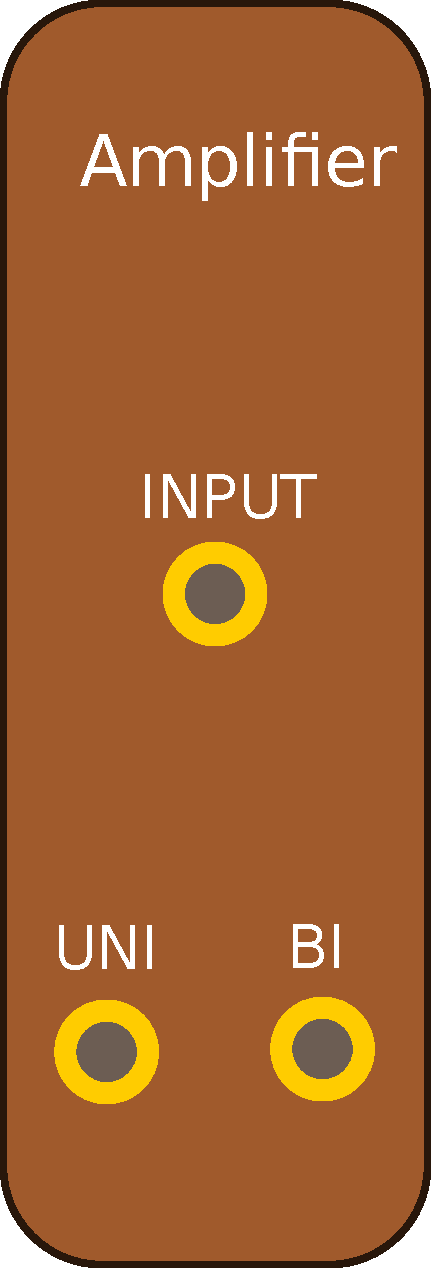
\includegraphics[height=0.25\textheight]{BilderAufbau/amp.pdf}
  
\includegraphics[height=0.25\textheight]{BilderAufbau/sca.pdf}
  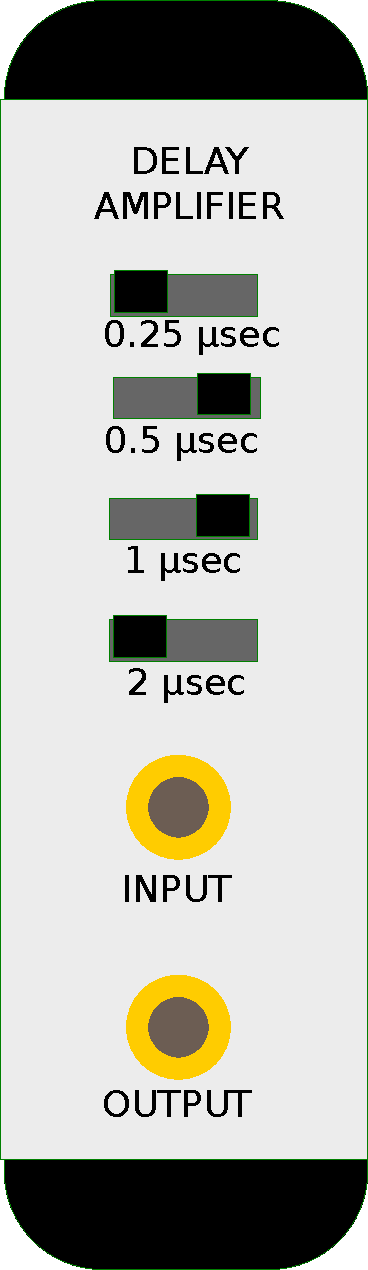
\includegraphics[height=0.25\textheight]{BilderAufbau/delay.pdf}
  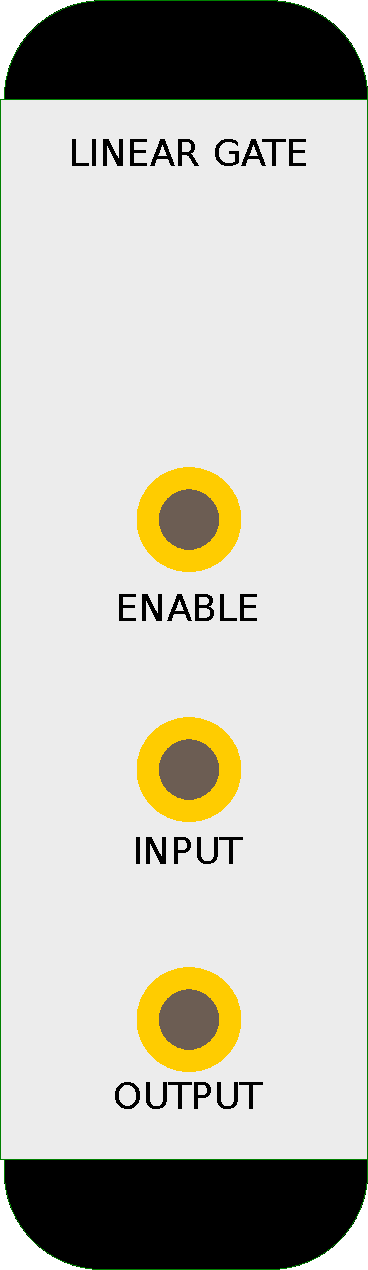
\includegraphics[height=0.25\textheight]{BilderAufbau/linear_gate.pdf}
  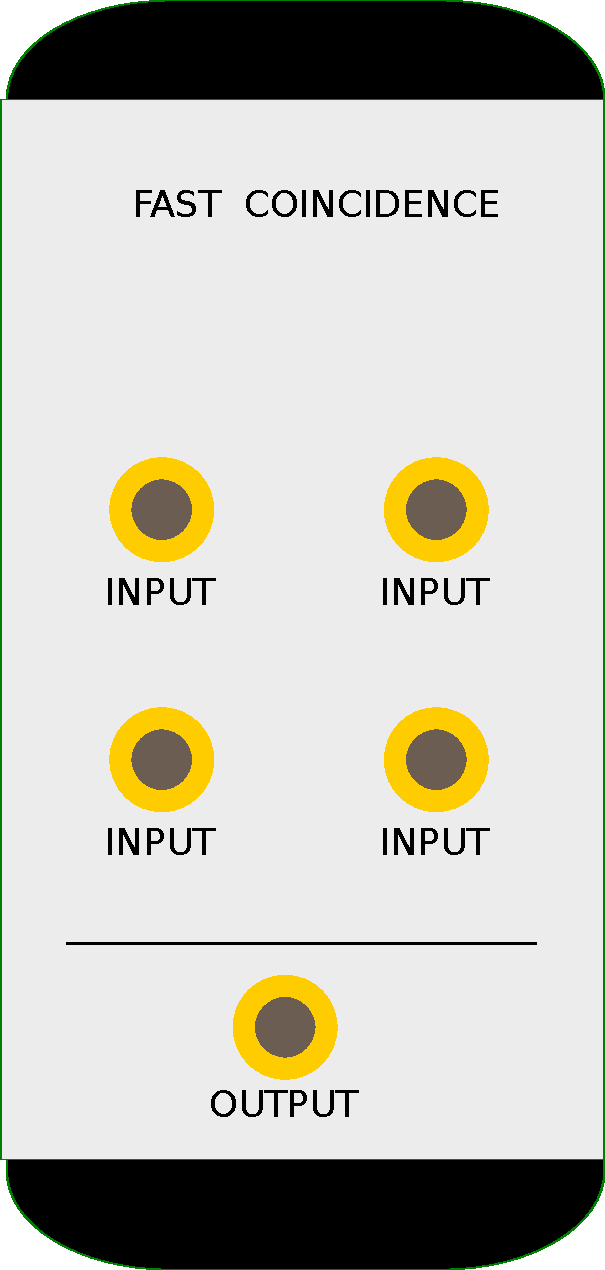
\includegraphics[height=0.25\textheight]{BilderAufbau/koinzidenz.pdf}
  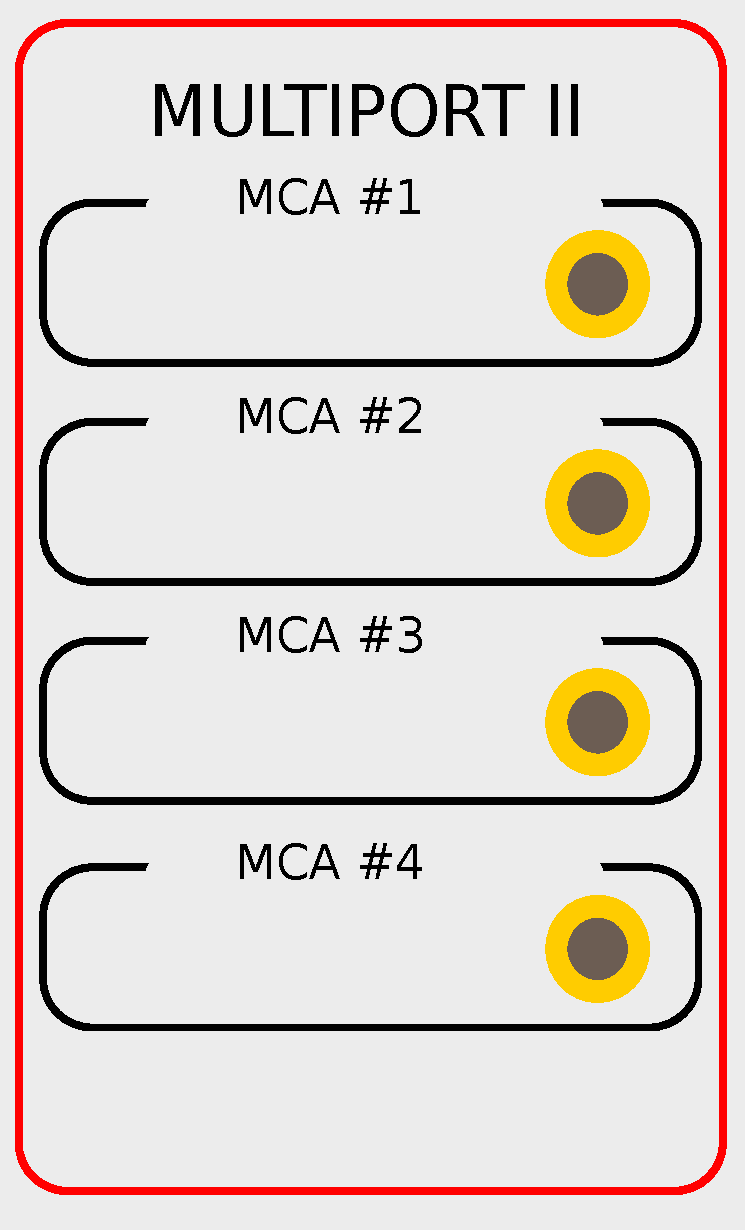
\includegraphics[height=0.25\textheight]{BilderAufbau/mca.pdf}
 \caption{Verstärker (Amp), Einkanalanalysator (SCA), Verzögerung (Delay), Gate, Koinzidenz, und Mehrkanalanalysator (von links)}
 \label{geraete}
\end{figure}



Wie bereits beschrieben geben die Szintillatoren für jedes Photon ein Signal aus, dessen Amplitude Rückschlüsse auf die Energie des Photons erlaubt. Der Verstärker integriert dieses Signal über die sogenannte "`shapping time"' um Rauschen zu unterdrücken. Weiterhin kann eine lineare Verstärkung des Signals eingestellt werden. Er besitzt zwei Ausgänge, die entweder ein unipolares oder ein bipolares Signal liefern. Dieses hat die Form der Lade- und Entladekurve des verwendeten Kondensators (Bipolar) bzw. dessen Betrag (Unipolar). Sollen nur Ereignisse einer bestimmten Energie weiterverarbeitet werden, kann man einen Single Channel Analyzer (SCA) verwenden. Bei diesem lässt sich eine minimale und maximale zulässige Energie einstellen (upper bzw. lower level) bei der ein neues Signal weitergeben werden soll. Über eine "`delay"' genannte Einstellung kann dieses über ein intrinsisches Minimum hinaus verzögert werden. Das ausgebene Signal hat die Form eines NIM-Standardsignals, also eine (neg.) Rechteckfunktion mit fest definierter Dauer und Amplitude. Da diese keine direkte Energieinformation mehr enthält, kann es nur zur Steuerung eines "`Gates"' oder als "`binäres"' Signal für eine Koinzidenzeinheit verwendet werden. Soll das eigentliche Energiesignal weiter untersucht werden, verwendet man das Signal des SCA als Auslöser für ein "`Linear Gate"'. Dieses Gate öffnet die Verbindung zwischen Input- und Output-Anschluß sobald es am Enable-Eingang ein NIM-Normsignal erhält für einen einstellbaren Zeitraum. Für ein gutes Signal-Rausch-Verhältnis sollte dieser recht kurz sein. Die Signallaufzeiten für das Enable- und das Energie-Signal dürfen daher nur minimal voneinander abweichen. Insbesondere muss das Energie-Signal verspätet gegenüber dem Enabler eintreffen, was durch ein weiteres Bauteil erreicht wird. Die Verzögerung (Delay) erlaubt es, eine grobe Verzögerung des Energiesignals vorzugeben. An diese kann dann das Enable-Signal angepasst werden. Das so gefilterte Signal kann nun von einem Mehrkanalanalysator aufgenommen werden und das resultierende Energiespektrum am PC betrachtet werden.

Soll die Gleichzeitigkeit von bis zu vier Signalen überprüft werden, kann anstelle mehrerer Gates auch eine Koinzidenzeinheit (Koinzidenz) verwendet werden. Diese überprüft ob in einem einstellbaren Zeitraum nach dem Eingang eines ersten Signals auch an allen anderen Eingängen Signale ankommen. Ist dies der Fall so wird am Ausgang ein Normsignal erzeugt.